% CO oxidation (LH): r ~ x b / (1 + x + b)^2 with x = K1 pCO, b = sqrt(K2 pO2) fixed.
% Maximum at x = 1 + b.
\documentclass[border=4pt]{standalone}
% Shared style for the ch. 10 schematic plots (figures/src/*.tex).
% Build one figure:  lualatex <name>.tex   then see README.md for the PNG step.
\usepackage{amsmath}
\usepackage{pgfplots}
\pgfplotsset{compat=1.18}
\usetikzlibrary{arrows.meta}

\definecolor{matblue}{HTML}{0072BD}
\definecolor{matorange}{HTML}{D95319}

\pgfplotsset{
  schematic/.style={
    width=8cm, height=6.2cm,
    axis lines=left,
    axis line style={-{Stealth[length=2.5mm]}, line width=0.8pt},
    xtick=\empty, ytick=\empty,
    xmin=0, ymin=0,
    clip=false,
    every axis x label/.style={at={(current axis.right of origin)}, anchor=north east, yshift=-4pt},
    every axis y label/.style={at={(current axis.above origin)}, anchor=north east, xshift=-4pt},
    label style={font=\normalsize},
    samples=200,
  },
  curve/.style={line width=1.4pt, color=matblue},
  guide/.style={line width=0.8pt, dashed, color=black!60},
}

\begin{document}
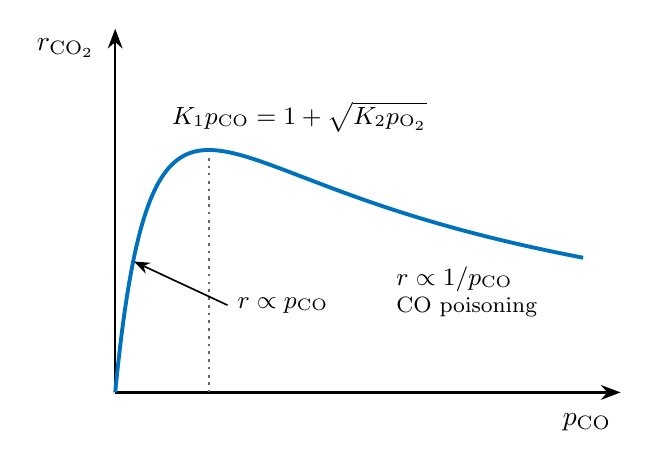
\begin{tikzpicture}
\begin{axis}[schematic, xmax=1.08, ymax=0.25,
    xlabel={$p_{\mathrm{CO}}$}, ylabel={$r_{\mathrm{CO_2}}$}]
  % b = 2, x = 15 p  ->  maximum at p = 0.2, r_max = 1/6
  \addplot[guide, dotted, domain=0:0.1667] (0.2, {x});
  \addplot[curve, domain=0:1] {2*15*x/(3+15*x)^2};
  \node[anchor=south west, font=\small, align=center] at (axis cs:0.1,0.172)
    {$K_1 p_{\mathrm{CO}} = 1 + \sqrt{K_2 p_{\mathrm{O_2}}}$};
  \draw[-{Stealth[length=2mm]}, line width=0.6pt] (axis cs:0.24,0.06) node[anchor=west, font=\small] {$r \propto p_{\mathrm{CO}}$} -- (axis cs:0.04,0.09);
  \node[anchor=south west, font=\small, align=left] at (axis cs:0.58,0.045)
    {$r \propto 1/p_{\mathrm{CO}}$\\[-1pt]\footnotesize CO poisoning};
\end{axis}
\end{tikzpicture}
\end{document}
